\documentclass[tikz,border=12pt]{standalone}
\usepackage[T1]{fontenc}
\usepackage{mathpazo}
\usepackage{amsmath,amssymb}
\usetikzlibrary{arrows.meta, calc}

\definecolor{stblue}{HTML}{7B97AD}
\definecolor{rwgold}{HTML}{B8995E}
\definecolor{sage}{HTML}{7A9A7E}
\definecolor{dkbrown}{HTML}{3D3530}
\definecolor{wmgray}{HTML}{7B7067}
\definecolor{cream}{HTML}{F9F6F0}
\definecolor{border}{HTML}{D4C9B8}
\definecolor{terracotta}{HTML}{C47A6A}
\definecolor{lavender}{HTML}{907EA0}

\begin{document}
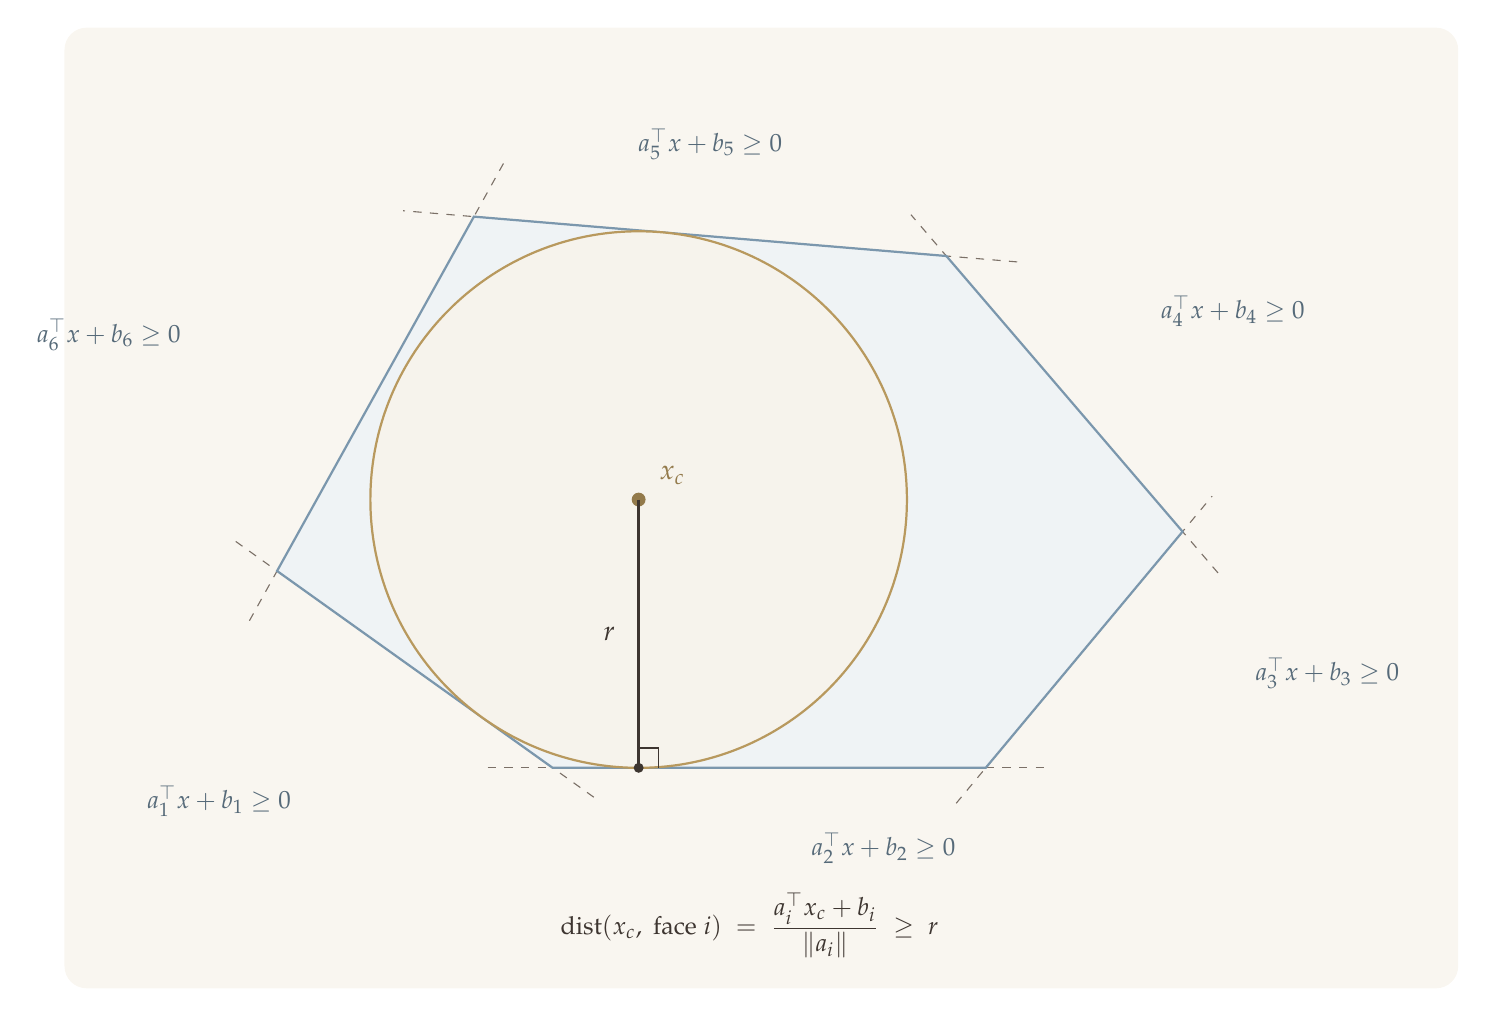
\begin{tikzpicture}[
    >={Stealth[length=3.5pt, width=2.5pt]},
    every node/.style={text=dkbrown},
  ]

  % ══════════════════════════════════════════════════════
  % Background
  % ══════════════════════════════════════════════════════
  \fill[cream, rounded corners=8pt] (-3.2,-2.8) rectangle (14.5,9.4);

  % ══════════════════════════════════════════════════════
  % Polygon vertices (elongated convex hexagon)
  % ══════════════════════════════════════════════════════
  % Chebyshev center: (4.092, 3.407), radius: 3.407
  % Tangent to E1 (lower-left), E2 (bottom), E5 (top)
  \coordinate (V1) at (-0.5, 2.5);
  \coordinate (V2) at (3.0, 0.0);
  \coordinate (V3) at (8.5, 0.0);
  \coordinate (V4) at (11.0, 3.0);
  \coordinate (V5) at (8.0, 6.5);
  \coordinate (V6) at (2.0, 7.0);

  \pgfmathsetmacro{\xcx}{4.092}
  \pgfmathsetmacro{\xcy}{3.407}
  \pgfmathsetmacro{\rad}{3.407}

  % ══════════════════════════════════════════════════════
  % Extended dashed halfspace lines (beyond vertices)
  % ══════════════════════════════════════════════════════
  \foreach \a/\b in {1/2, 2/3, 3/4, 4/5, 5/6, 6/1}{
    \draw[wmgray, thin, dashed]
      ($(V\a)!-0.15!(V\b)$) -- ($(V\b)!-0.15!(V\a)$);
  }

  % ══════════════════════════════════════════════════════
  % Filled polytope
  % ══════════════════════════════════════════════════════
  \fill[stblue!12]
    (V1) -- (V2) -- (V3) -- (V4) -- (V5) -- (V6) -- cycle;
  \draw[stblue, thick]
    (V1) -- (V2) -- (V3) -- (V4) -- (V5) -- (V6) -- cycle;

  % ══════════════════════════════════════════════════════
  % Inscribed circle (Chebyshev ball)
  % ══════════════════════════════════════════════════════
  \fill[rwgold!12] (\xcx, \xcy) circle (\rad);
  \draw[rwgold, thick] (\xcx, \xcy) circle (\rad);

  % ══════════════════════════════════════════════════════
  % Center point and label
  % ══════════════════════════════════════════════════════
  \fill[rwgold!80!black] (\xcx, \xcy) circle (2.5pt);
  \node[rwgold!80!black, font=\normalsize, anchor=south west,
        xshift=4pt, yshift=2pt]
    at (\xcx, \xcy) {$x_c$};

  % ══════════════════════════════════════════════════════
  % Radius to Edge 2 (bottom, tangent, horizontal)
  % ══════════════════════════════════════════════════════
  % E2: V2(3,0)->V3(8.5,0), horizontal, n_hat=(0,1)
  % Foot: (4.092, 0.0)
  \coordinate (foot2) at (4.092, 0.0);

  \draw[dkbrown, line width=1.2pt] (\xcx, \xcy) -- (foot2);
  \node[dkbrown, font=\normalsize, anchor=east, xshift=-5pt]
    at ($(\xcx,\xcy)!0.5!(foot2)$) {$r$};
  \fill[dkbrown] (foot2) circle (1.8pt);

  % Right-angle mark at foot (edge is horizontal, normal is vertical)
  \draw[dkbrown, line width=0.6pt]
    ($(foot2)+(0.25,0)$) -- ++(0, 0.25) -- ++(-0.25, 0);

  % ══════════════════════════════════════════════════════
  % Halfspace labels  a_i^T x + b_i >= 0
  % All labels horizontal for readability, placed outside the polygon
  % ══════════════════════════════════════════════════════

  % E1: V1->V2, lower-left edge
  \node[stblue!70!black, font=\small, anchor=north east]
    at (-0.2, -0.1) {$a_1^\top x + b_1 \geq 0$};

  % E2: V2->V3, bottom edge, horizontal
  \node[stblue!70!black, font=\small, anchor=north]
    at (7.2, -0.7) {$a_2^\top x + b_2 \geq 0$};

  % E3: V3->V4, lower-right edge
  \node[stblue!70!black, font=\small, anchor=west]
    at (11.8, 1.2) {$a_3^\top x + b_3 \geq 0$};

  % E4: V4->V5, upper-right edge
  \node[stblue!70!black, font=\small, anchor=west]
    at (10.6, 5.8) {$a_4^\top x + b_4 \geq 0$};

  % E5: V5->V6, top edge, nearly horizontal
  \node[stblue!70!black, font=\small, anchor=south]
    at (5.0, 7.6) {$a_5^\top x + b_5 \geq 0$};

  % E6: V6->V1, upper-left edge
  \node[stblue!70!black, font=\small, anchor=east]
    at (-1.6, 5.5) {$a_6^\top x + b_6 \geq 0$};

  % ══════════════════════════════════════════════════════
  % Distance formula annotation
  % ══════════════════════════════════════════════════════
  \node[dkbrown, font=\small, align=center]
    at (5.5, -2.0)
    {$\displaystyle\mathrm{dist}(x_c,\;\text{face}\;i)
      \;=\; \frac{a_i^\top x_c + b_i}{\|a_i\|}
      \;\geq\; r$};

\end{tikzpicture}
\end{document}
